\documentclass{fizykalab}

% Ustawienia do tabelki

\wydzial{WI}
\autorjeden{Dawid Komęza}
\autordwa{Magdalena Śmietana}
\rok{II}
\grupa{14}
\zespol{2}
\temat{Moduł Younga}
\nrcwiczenia{11}
\datawykonania{11.10.2025}
\dataoddaniajeden{}
\zwrotdopoprawy{}
\dataoddaniadwa{}
\datazaliczenia{}

\begin{document}

\maketitle

\section{Cel ćwiczenia}

Celem ćwiczenia jest wyznaczenie modułu Younga \(E\) metodą statyczną
na podstawie pomiaru wydłużenia drutu z badanego metalu obciążonego
znaną siłą. Dodatkowo celem jest weryfikacja liniowej zależności prawa
Hooke'a w zakresie odkształceń sprężystych oraz oszacowanie niepewności
wyniku i porównanie go z wartościami tablicowymi. W szczególności:

\begin{itemize}
  \item wykonanie pomiarów dla dwóch drutów wykonanych z różnych metali,
    z zachowaniem dopuszczalnych obciążeń (do 10 kg dla stali, do 6 kg dla mosiądzu);
  \item zapis wskazań czujnika dla rosnących \(\uparrow\) i malejących
    \(\downarrow\) wartości obciążenia oraz wyznaczenie wydłużenia
    drutu \(\Delta l\) z uwzględnieniem przełożenia dźwigni czujnika,
    tj. \(\Delta l = (\text{cz} \uparrow + \text{cz} \downarrow)/4\);
  \item porównanie otrzymanych wartości \(E\) z danymi tablicowymi dla
    badanych materiałów, ocena zgodności w granicach niepewności
    rozszerzonej i określenie wniosków dotyczących pomiarów i wyników.
\end{itemize}

\section{Wstęp teoretyczny}

Podstawą opisu sprężystego odkształcania ciał stałych jest prawo Hooke'a,
które w zakresie małych odkształceń (zakres liniowo-sprężysty) opisuje
proporcjonalną zależność między naprężeniem a odkształceniem względnym.
Dla jednoosiowego rozciągania (pręt lub drut obciążony siłą wzdłuż osi)
prawo Hooke'a ma postać liniową:
$$
\sigma = E\,\varepsilon,
$$
gdzie: \( \sigma \) to naprężenie normalne, \( \varepsilon \) to
odkształcenie względne, a \( E \) to moduł Younga (moduł sprężystości
podłużnej). Naprężenie definiuje się jako siłę odniesioną do pola
przekroju poprzecznego próbki,
\( \sigma = F/S \), natomiast odkształcenie względne jako stosunek
wydłużenia do długości początkowej,
\( \varepsilon = \Delta l / l \).

Stąd moduł Younga można wyrazić wzorem:
$$
E = \frac{\sigma}{\varepsilon} = \frac{F/S}{\Delta l / l}
= \frac{F\,l}{S\,\Delta l}.
$$

W ćwiczeniu wyznacza się \( E \) metodą statyczną, mierząc wydłużenie
prostego drutu o długości \( l \) i średnicy
\( d \), rozciąganego siłą \( F \). Dla kołowego przekroju
\( S = \pi d^{2}/4 \) otrzymać można wzór roboczy:
$$
E = \frac{4\,F\,l}{\pi\,d^{2}\,\Delta l}.
$$
Siłę rozciągającą oblicza się z masy odważników:
\( F = m\,g \), gdzie \( g \) jest przyspieszeniem ziemskim.

\bigskip
Zgodnie z prawem Hooke'a, w zakresie sprężystym zależność
\( \Delta l(F) \) powinna być liniowa i można ją opisać równaniem
prostej \( \Delta l = a\,F + b \), gdzie \( a = l/(E\,S) \).
Uwzględniając poprzednie wzory, moduł Younga można wyrazić jako:
$$
E = \frac{l}{a\,S} = \frac{4\,l}{\pi\,d^{2}\,a}.
$$

Punkty zauważalnie odstające od przebiegu liniowego świadczą o
niedoskonałościach układu (tarcie, luz, histereza czujnika) lub o
opuszczeniu ścisłego zakresu sprężystości (deformacja plastyczna). Aby ograniczyć wpływ tych
czynników, rejestruje się wskazania przy obciążaniu i odciążaniu oraz
uśrednia się je.

W zastosowanym układzie czujnik mikrometryczny współpracuje z dźwignią,
która przenosi ruch końca drutu na czujnik. Ze względu na przełożenie
mechaniczne wskazanie czujnika jest dwukrotnie większe od rzeczywistego
wydłużenia drutu. Dlatego przy wyznaczaniu wydłużenia wykorzystuje się
średnią ze wskazań dla narastającego i malejącego obciążenia oraz dzieli
się wynik dodatkowo przez 2, co prowadzi do praktycznego wzoru
uśredniającego:
$$
\Delta l = \frac{\text{cz} \uparrow + \text{cz} \downarrow}{4},
$$
gdzie \( \text{cz} \uparrow \) i \( \text{cz} \downarrow \) oznaczają
odczyty czujnika odpowiednio przy dokładaniu i zdejmowaniu odważników.

Moduł Younga ma wymiar i jednostkę ciśnienia: \( [E] = \mathrm{Pa} \).
Dla metali typowe wartości mieszczą się w przedziale od kilkudziesięciu
do kilkuset gigapaskali (np. stal około \( 200\ \mathrm{GPa} \),
  miedź około \( 110\ \mathrm{GPa} \), mosiądz około \( 90\text{--}110\
\mathrm{GPa} \)). Przekroczenie granicy sprężystości prowadzi do
odkształceń trwałych (nieliniowość, uplastycznienie), a proste zależności
powyżej przestają obowiązywać. Dlatego w trakcie ćwiczenia należy dobierać
obciążenia w takim zakresie, aby materiał pracował sprężyście, a wykres
\( \Delta l(F) \) pozostawał liniowy.

\section{Wzory}

\subsection{Definicje i zależności podstawowe}

Podstawą wyznaczenia modułu Younga jest prawo Hooke'a, określające
zależność między naprężeniem a odkształceniem względnym:
$$
\sigma = E\,\varepsilon,
$$
gdzie \( \sigma \) oznacza naprężenie (czyli siłę odniesioną do jednostki
powierzchni przekroju), \( \varepsilon \) to odkształcenie względne, a
\( E \) to poszukiwany moduł Younga.

Aby wyrazić naprężenie i odkształcenie w postaci praktycznej,
korzystamy z definicji:
$$
\sigma = \frac{F}{S}, \qquad \varepsilon = \frac{\Delta l}{l},
$$
gdzie \( F \) to przyłożona siła rozciągająca, \( S \) — pole przekroju
poprzecznego drutu, \( \Delta l \) — jego wydłużenie, a \( l \) — długość
początkowa odcinka pomiarowego.

Podstawiając te zależności do prawa Hooke'a, otrzymujemy wyrażenie na
moduł Younga:
$$
E = \frac{\sigma}{\varepsilon}
= \frac{F l}{S\,\Delta l}.
$$
Z równania tego wynika, że im większe jest wydłużenie drutu dla tej samej
siły, tym mniejszy moduł sprężystości (materiał bardziej podatny na
odkształcenie).
\pagebreak

\subsection{Zależność pomiarowa i wzór roboczy}

Na podstawie prawa Hooke'a można przewidzieć, że w zakresie sprężystym
zależność wydłużenia drutu od przyłożonej siły powinna być liniowa.
Można ją opisać równaniem prostej:
$$
\Delta l(F) = a\,F + b.
$$
Współczynnik \( a \) jest nachyleniem prostej, wyznaczonym z wykresu
\(\Delta l(F)\), natomiast \( b \) reprezentuje ewentualne przesunięcie
(luz początkowy lub błąd zerowania).
Przekształcając wzór na moduł Younga, otrzymujemy zależność:
$$
\Delta l = \frac{F\,l}{E\,S}
$$
co pozwala zidentyfikować współczynnik nachylenia:
$$
a = \frac{l}{E\,S},
$$
co po przekształceniu daje wzór roboczy na moduł Younga:
$$
E = \frac{l}{a\,S}.
$$

\subsection{Wzory pomocnicze}

Ze względu na zastosowanie w układzie dźwigni, czujnik mikrometryczny
pokazuje odkształcenie dwukrotnie większe niż rzeczywiste. Dodatkowo dla
zmniejszenia wpływu histerezy pomiary wykonuje się przy obciążaniu
(\(\uparrow\)) i odciążaniu (\(\downarrow\)), a następnie uśrednia:
$$
\Delta l = \frac{\text{cz} \uparrow + \text{cz} \downarrow}{4}.
$$
Taki sposób przeliczenia eliminuje systematyczne błędy
mechaniczne przyrządu.

\bigbreak
Podczas pomiaru średnicy drutu stosuje się trzy niezależne pomiary w
różnych miejscach, by uwzględnić ewentualne nierówności powierzchni.
Średnią średnicę obliczamy ze wzoru:
$$
\overline{d} = \frac{d_{1}+d_{2}+d_{3}}{3}.
$$

Drut badany w ćwiczeniu ma przekrój kołowy, dlatego pole przekroju można
zapisać jako:
$$
S = \frac{\pi d^{2}}{4},
$$
gdzie \( d \) to średnica drutu.

Ponieważ napięcie w drucie powstaje w wyniku przyłożonej masy \( m \)
odważników, siła rozciągająca wynosi:
$$
F = m\,g,
$$
gdzie \( g \) to przyspieszenie ziemskie (\( g \approx 9{,}811\,\mathrm{m/s^2} \)).
W ten sposób uzyskujemy zależność pomiędzy masą użytych odważników a
siłą działającą na drut.

\subsection{Niepewności i niepewność rozszerzona}

Niepewności pomiarowe przenosi się na wynik modułu Younga zgodnie
z prawem przenoszenia niepewności względnych. Dla obliczeń opartych
o nachylenie prostej \(a\) otrzymujemy:
$$
\frac{u_{c}(E)}{E} =
\sqrt{
  \left(\frac{u(l)}{l}\right)^{2} +
  \left(2\,\frac{u(d)}{d}\right)^{2} +
  \left(\frac{u(a)}{a}\right)^{2}
}.
$$
Niepewność rozszerzoną oblicza się jako:
$$
U(E) = k\,u_{c}(E),
$$
gdzie \(k\) to współczynnik rozszerzenia, przyjmowany najczęściej
\(k \approx 2\).

Taka procedura pozwala określić, czy uzyskany wynik modułu Younga jest
zgodny (w granicach niepewności rozszerzonej) z wartością tablicową dla
danego materiału.

\subsection{Konwersje jednostek i stałe}

Ponieważ pomiary wykonywane są w milimetrach, konieczne jest
przeliczenie jednostek na metry w układzie SI:
$$
\Delta l[\mathrm{m}] = \Delta l[\mathrm{mm}] \cdot 10^{-3}, \qquad
d[\mathrm{m}] = d[\mathrm{mm}] \cdot 10^{-3}.
$$
Przyspieszenie ziemskie przyjmujemy jako:
$$
g \approx 9{,}811\,\mathrm{m/s^2}.
$$
Po uwzględnieniu tych konwersji wszystkie wzory przyjmują poprawną
postać w układzie SI, a otrzymane wartości modułu Younga będą wyrażone
w paskalach \([E] = \mathrm{Pa}\).

\subsection{Wartości tablicowe modułu Younga i innych stałych sprężystych}

Dla porównania wyników pomiarów z wartościami literaturowymi w tabeli
poniżej zestawiono orientacyjne wartości modułu Younga \(E\), modułu
Kirchoffa \(G\) (modułu sztywności postaciowej) oraz granicy plastyczności
lub naprężenia dopuszczalnego \(\sigma_s\) dla wybranych materiałów.
Wszystkie wartości podano w gigapaskalach \([\mathrm{GPa}]\).

\bigskip
\begin{center}
  \begin{tabular}{|l|c|c|c|}
    \hline
    \textbf{Materiał} & \textbf{\(E\) [GPa]} & \textbf{\(G\) [GPa]} & \textbf{\(\sigma_s\) [GPa]} \\
    \hline
    Guma & 0{,}001 & 0{,}00002 & 0{,}001 \\
    \hline
    Ołów & 17 & 5{,}9 -- 6{,}4 & -- \\
    \hline
    Aluminium & 70 & 26 & 0{,}24 (dural) \\
    \hline
    Miedź & 110 -- 130 & 38 & 0{,}07 \\
    \hline
    Mosiądz & 100 & 42 & 0{,}3 \\
    \hline
    Stal węglowa pospolita & 210 -- 220 & 78 -- 82 & 0{,}4 \\
    \hline
    Stal węglowa sprężynowa & jw. & jw. & 1{,}65 \\
    \hline
    Diament & 1200 & 480 & -- \\
    \hline
  \end{tabular}
\end{center}

\bigskip
Moduł Younga ma bardzo szeroki zakres wartości — od około
\(10^{-3}\ \mathrm{GPa}\) dla gumy (materiału bardzo podatnego) aż do
ponad \(10^{3}\ \mathrm{GPa}\) dla diamentu, będącego jednym z
najsztywniejszych znanych materiałów. Bardzie typowe materiały konstrukcyjne,
takie jak stal, aluminium czy mosiądz, mają moduły Younga w
zakresie od około \(70\ \mathrm{GPa}\) (aluminium) do ponad
\(200\ \mathrm{GPa}\) (stal). Pomiar laboratoryjny powinien więc dać wynik
zbliżony do tych wartości.

\pagebreak
\section{Aparatura pomiarowa}

Zastosowana metoda pomiaru modułu Younga opiera się na bezpośrednim
wyznaczeniu wielkości występujących we wzorze definicyjnym:
\( E = \dfrac{F\,l}{S\,\Delta l} \).
Do realizacji pomiarów zbudowano stanowisko przedstawione schematycznie
na rysunku~\ref{rys:uklad}. Układ ten umożliwia precyzyjny pomiar
wydłużenia drutu w funkcji przyłożonej siły rozciągającej.

\begin{figure}[h!]
  \centering
  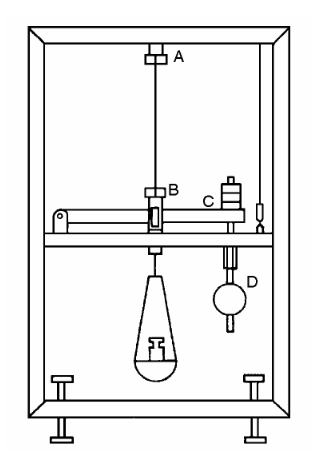
\includegraphics[width=0.6\textwidth]{rys1.png}
  \caption{Urządzenie do pomiaru modułu Younga metodą statyczną.}
  \label{rys:uklad}
\end{figure}

\begin{itemize}
  \item \textbf{A – Górny uchwyt:} służy do sztywnego zamocowania
    badanego drutu w statywie. Jest stabilnym punktem odniesienia,
    względem którego mierzone jest wydłużenie drutu.
  \item \textbf{B – Dolny uchwyt:} połączony jest z szalką, na której
    umieszcza się odważniki. Przekazuje on siłę ciężkości obciążników
    na drut, powodując jego rozciąganie.
  \item \textbf{C – Dźwignia pomiarowa:} przekazuje ruch (wydłużenie)
    dolnego końca drutu do czujnika mikrometrycznego. Jest
    podparta w połowie długości, natomiast punkt połączenia z drutem
    oraz punkt styku z czujnikiem znajdują się symetrycznie po obu
    stronach osi obrotu. Z tego względu przełożenie mechaniczne
    dźwigni wynosi 2:1, co oznacza, że czujnik wskazuje wartość
    dwukrotnie większą niż rzeczywiste wydłużenie drutu.
  \item \textbf{D - Czujnik mikrometryczny:} służy do pomiaru
    przemieszczenia końca dźwigni z dokładnością 0{,}01 mm.
    Wskazania czujnika uśrednia się dla cyklu obciążania i
    odciążania, aby zredukować wpływ tarcia i ewentualnej histerezy.
\end{itemize}

Średnicę badanego drutu \(d\) mierzy się niezależnie \emph{mikrometrem
śrubowym}, wykonując pomiary w trzech różnych miejscach rozłożonych na
jego długości. Na podstawie tych pomiarów oblicza się średnią wartość
średnicy \(\overline{d}\).

\pagebreak

\section{Wyniki pomiarów dla drutu stalowego}

W tej części ćwiczenia badano zależność wydłużenia \(\Delta l\) od siły
rozciągającej \(F\) dla drutu stalowego. Długość odcinka pomiarowego
wynosiła \(l = 1{,}075\ \mathrm{m}\) przy niepewności
\(u(l)=2\ \mathrm{mm}\). Średnicę zmierzono trzykrotnie:
\(d_1=0{,}75\ \mathrm{mm},\ d_2=0{,}77\ \mathrm{mm},\ d_3=0{,}76\ \mathrm{mm}\);
przyjęto \(\overline{d}=0{,}76\ \mathrm{mm}=0{,}00076\ \mathrm{m}\) oraz
\(u(d)=0{,}01\ \mathrm{mm}\).
Wydłużenie wyznaczano ze wskazań czujnika metodą
\(\Delta l = (\mathrm{cz}\uparrow + \mathrm{cz}\downarrow)/4\).

\begin{table}[H]
  \centering
  \caption{Pomiary wydłużenia drutu stalowego dla kolejnych obciążeń.}
  \begin{tabular}{ccccccc}
    \toprule
    Lp. & \(m\)\,[kg] & \(F\)\,[N] &
    cz \(\uparrow\)\,[mm] & cz \(\downarrow\)\,[mm] &
    \(\Delta l\)\,[mm] & \(\Delta l\)\,[m] \\
    \midrule
    1 & 1 & 9{,}811 & 0{,}96 & 1{,}11 & 0{,}5175 & 0{,}0005175 \\
    2 & 2 & 19{,}622 & 1{,}62 & 1{,}72 & 0{,}8350 & 0{,}0008350 \\
    3 & 3 & 29{,}433 & 1{,}99 & 2{,}08 & 1{,}0175 & 0{,}0010175 \\
    4 & 4 & 39{,}244 & 2{,}43 & 2{,}38 & 1{,}2025 & 0{,}0012025 \\
    5 & 5 & 49{,}055 & 2{,}61 & 2{,}76 & 1{,}3425 & 0{,}0013425 \\
    6 & 6 & 58{,}866 & 3{,}04 & 3{,}04 & 1{,}5200 & 0{,}0015200 \\
    7 & 7 & 68{,}677 & 3{,}24 & 3{,}40 & 1{,}6600 & 0{,}0016600 \\
    8 & 8 & 78{,}488 & 3{,}57 & 3{,}64 & 1{,}8025 & 0{,}0018025 \\
    9 & 9 & 88{,}299 & 3{,}78 & 3{,}92 & 1{,}9250 & 0{,}0019250 \\
    \bottomrule
  \end{tabular}
  \label{tab:stal_pomiary}
\end{table}

\begin{figure}[H]
  \centering
  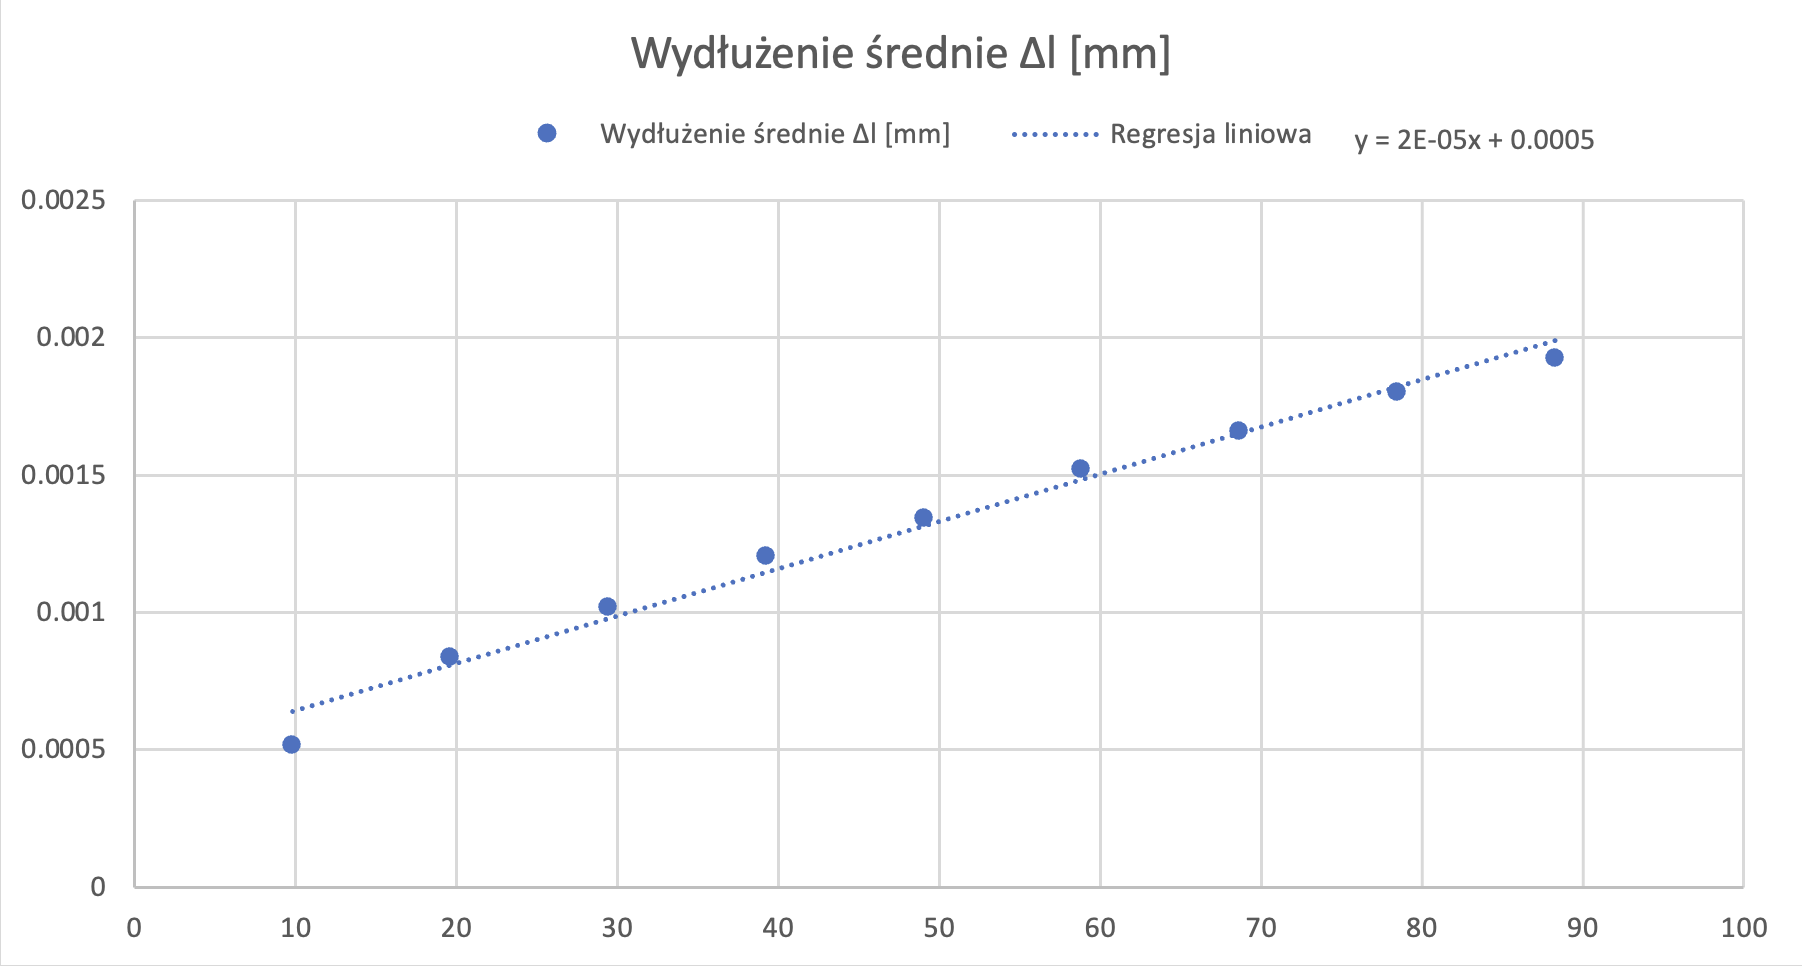
\includegraphics[width=0.9\textwidth]{stal.png}
  \caption{Wykres zależności wydłużenia drutu stalowego od przyłożonej siły.
  Do punktów dopasowano prostą metodą najmniejszych kwadratów.}
  \label{rys:uklad_stal}
\end{figure}

Dopasowanie liniowe zależności \(\Delta l(F) = a\,F + b\) wykonano w
programie Microsoft Excel (\texttt{REGLINP/LINEST}).
Otrzymano nachylenie:
$$
a = (1{,}7217 \pm 0{,}0082)\times 10^{-5}\ \mathrm{\tfrac{m}{N}},
$$
gdzie podana niepewność to \(u(a)\).

\subsection{Wyznaczenie modułu Younga}

Korzystając z zależności \(E = \dfrac{4\,l}{\pi\,d^{2}\,a}\) oraz
\(l = 1{,}075\ \mathrm{m},\ d=0{,}00076\ \mathrm{m},\
a = 1{,}7217\times 10^{-5}\ \mathrm{m/N}\), otrzymano:
$$
E = \frac{4 \cdot 1{,}075}{\pi \cdot (0{,}00076)^2 \cdot
1{,}7217\times 10^{-5}}
= 1{,}37636\times 10^{11}\ \mathrm{Pa}
= 137{,}6\ \mathrm{GPa}.
$$

\subsection{Niepewność i wynik końcowy}

Względne niepewności wielkości wejściowych:
$$
\frac{u(l)}{l}=\frac{0{,}002}{1{,}075}=0{,}00186,\qquad
\frac{u(d)}{d}=\frac{0{,}00001}{0{,}00076}=0{,}01316,\qquad
\frac{u(a)}{a}=\frac{8{,}194\times10^{-7}}{1{,}7217\times10^{-5}}
=0{,}04760.
$$
Prawo przenoszenia niepewności względnych dla
\(E = 4l/(\pi d^{2}a)\) daje:
$$
\left(\frac{u(E)}{E}\right)^2 =
(0{,}00186)^2 + \bigl(2\cdot 0{,}01316\bigr)^2 + (0{,}04760)^2
= 0{,}002963,
$$
stąd
$$
\frac{u(E)}{E} = 0{,}05442
\quad\Rightarrow\quad
u(E) = 0{,}05442 \cdot 1{,}37636\times10^{11}
= 7{,}49\times10^{9}\ \mathrm{Pa}.
$$
Dla współczynnika rozszerzenia \(k=2\):
$$
U(E) = 2\,u(E) = 1{,}50\times10^{10}\ \mathrm{Pa} = 15{,}0\ \mathrm{GPa}.
$$

\subsection*{Wynik końcowy}
$$
\boxed{E = (1{,}376 \pm 0{,}075)\times 10^{11}\ \mathrm{Pa}
= (137{,}6 \pm 7{,}5)\ \mathrm{GPa}}
$$
% k = 2 (niepewność rozszerzona)
$$
\boxed{E = (137{,}6 \pm 15{,}0)\ \mathrm{GPa}\quad (k=2)}
$$

Porównując z wartością tablicową dla stali \(E_t \approx 210\ \mathrm{GPa}\),
stwierdzamy, że wynik \textbf{nie jest zgodny} w granicach niepewności rozszerzonej:
$$
|E_t - E| = |210 - 137{,}6| = 72{,}4\ \mathrm{GPa} > U(E) = 15{,}0\ \mathrm{GPa}.
$$

\subsection{Uwagi i wnioski}

Otrzymany wynik jest znacznie mniejszy od wartości tablicowej.
Prawdopodobną przyczyną jest fakt, że drut stalowy był mocno
wyeksploatowany i w początkowej fazie obciążenia zamiast do wydłużania
dochodziło do prostowania. W efekcie początkowe odkształcenia były
znacznie większe niż wynikałoby to z prawa Hooke'a, co skutkowało
zaniżeniem wyznaczonego modułu Younga. Dodatkowo, pomiary
mogły być obarczone błędami wynikającymi z dużego tarcia w układzie
dźwigni i czujnika, a także z niedokładności w pomiarze średnicy drutu.

\pagebreak

\section{Wyniki pomiarów dla drutu mosiężnego}

W tej części ćwiczenia badano zależność wydłużenia \(\Delta l\) od siły
rozciągającej \(F\) dla drutu mosiężnego. Długość odcinka pomiarowego
wynosiła \(l = 1{,}068\ \mathrm{m}\) przy niepewności
\(u(l)=2\ \mathrm{mm}\). Średnicę zmierzono trzykrotnie:
\(d_1=1{,}17\ \mathrm{mm},\ d_2=1{,}20\ \mathrm{mm},\ d_3=1{,}17\ \mathrm{mm}\);
przyjęto \(\overline{d}=1{,}18\ \mathrm{mm}=0{,}00118\ \mathrm{m}\) oraz
\(u(d)=0{,}01\ \mathrm{mm}\).
Wydłużenie wyznaczano ze wskazań czujnika metodą
\(\Delta l = (\mathrm{cz}\uparrow + \mathrm{cz}\downarrow)/4\).

\begin{table}[H]
  \centering
  \caption{Pomiary wydłużenia drutu mosiężnego dla kolejnych obciążeń.}
  \begin{tabular}{ccccccc}
    \toprule
    Lp. & \(m\)\,[kg] & \(F\)\,[N] &
    cz \(\uparrow\)\,[mm] & cz \(\downarrow\)\,[mm] &
    \(\Delta l\)\,[mm] & \(\Delta l\)\,[m] \\
    \midrule
    1 & 1 & 9{,}811 & 0{,}61 & 0{,}68 & 0{,}3225 & 0{,}0003225 \\
    2 & 2 & 19{,}622 & 1{,}01 & 1{,}06 & 0{,}5175 & 0{,}0005175 \\
    3 & 3 & 29{,}433 & 1{,}33 & 1{,}44 & 0{,}6925 & 0{,}0006925 \\
    4 & 4 & 39{,}244 & 1{,}67 & 1{,}70 & 0{,}8425 & 0{,}0008425 \\
    5 & 5 & 49{,}055 & 1{,}85 & 1{,}98 & 0{,}9575 & 0{,}0009575 \\
    \bottomrule
  \end{tabular}
  \label{tab:mos_pomiary}
\end{table}

\begin{figure}[H]
  \centering
  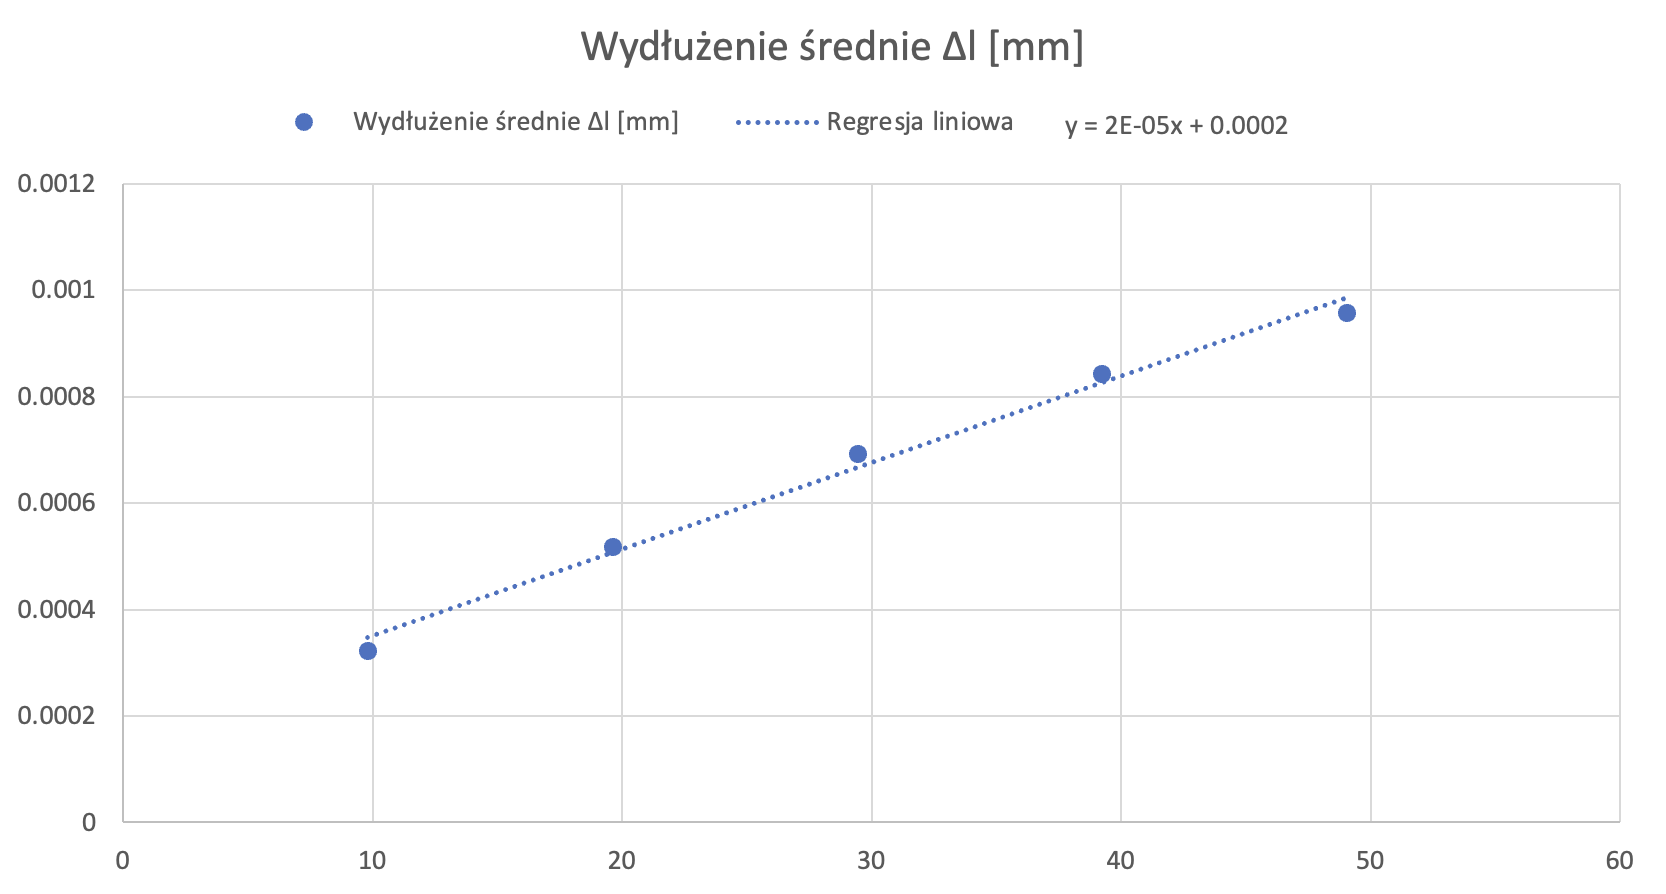
\includegraphics[width=0.9\textwidth]{mosiadz.png}
  \caption{Wykres zależności wydłużenia drutu mosiężnego od przyłożonej siły.
  Do punktów dopasowano prostą metodą najmniejszych kwadratów.}
  \label{rys:uklad_mos}
\end{figure}

Dopasowanie liniowe zależności \(\Delta l(F) = a\,F + b\) wykonano w
programie Microsoft Excel (\texttt{REGLINP/LINEST}).
Otrzymano nachylenie:
$$
a = (1{,}6257 \pm 0{,}0924)\times 10^{-5}\ \mathrm{\tfrac{m}{N}},
$$
gdzie podana niepewność to \(u(a)=9{,}24389\times 10^{-7}\ \mathrm{m/N}\).

\subsection{Wyznaczenie modułu Younga}

Korzystając z zależności \(E = \dfrac{4\,l}{\pi\,d^{2}\,a}\) oraz
\(l = 1{,}068\ \mathrm{m},\ d=0{,}00118\ \mathrm{m},\
a = 1{,}62573\times 10^{-5}\ \mathrm{m/N}\), otrzymano:
$$
E = \frac{4 \cdot 1{,}068}{\pi \cdot (0{,}00118)^2 \cdot
1{,}62573\times 10^{-5}}
= 6{,}0072\times 10^{10}\ \mathrm{Pa}
= 60{,}07\ \mathrm{GPa}.
$$

\pagebreak

\subsection{Niepewność i wynik końcowy}

Względne niepewności wielkości wejściowych:
$$
\frac{u(l)}{l}=\frac{0{,}002}{1{,}068}=0{,}00187,\qquad
\frac{u(d)}{d}=\frac{0{,}00001}{0{,}00118}=0{,}00847,\qquad
\frac{u(a)}{a}=\frac{9{,}24389\times10^{-7}}{1{,}62573\times10^{-5}}
=0{,}0569.
$$
Prawo przenoszenia niepewności względnych dla
\(E = 4l/(\pi d^{2}a)\) daje:
$$
\left(\frac{u(E)}{E}\right) =
\sqrt{(0{,}00187)^2 + \bigl(2\cdot 0{,}00847\bigr)^2 + (0{,}0569)^2}
= 0{,}0594,
$$
stąd
$$
u(E) = 0{,}0594 \cdot 6{,}0072\times10^{10}
= 3{,}57\times10^{9}\ \mathrm{Pa}
= 3{,}57\ \mathrm{GPa}.
$$
Dla współczynnika rozszerzenia \(k=2\):
$$
U(E) = 2\,u(E) = 7{,}14\times10^{9}\ \mathrm{Pa}
= 7{,}14\ \mathrm{GPa}.
$$

\subsection*{Wynik końcowy}
% k = 1 (niepewność standardowa)
$$
\boxed{E = (6{,}01 \pm 0{,}36)\times 10^{10}\ \mathrm{Pa}
= (60{,}07 \pm 3{,}57)\ \mathrm{GPa}}
$$
% k = 2 (niepewność rozszerzona)
$$
\boxed{E = (60{,}07 \pm 7{,}14)\ \mathrm{GPa}\quad (k=2)}
$$

\subsection{Ocena zgodności i uwagi}

Literaturowo dla mosiądzu podaje się \(E \approx 90\text{--}110\ \mathrm{GPa}\).
Otrzymany wynik \(E = 60{,}1\ \mathrm{GPa}\) jest istotnie mniejszy:
różnica względem dolnej granicy \(90\ \mathrm{GPa}\) wynosi
\(29{,}9\ \mathrm{GPa} > U(E)=7{,}14\ \mathrm{GPa}\),
zatem wynik \textbf{nie jest zgodny} w granicach niepewności
rozszerzonej. Możliwe przyczyny:
- zawyżony pomiar średnicy \(d\) (E zależy jak \(1/d^{2}\));
- zwiększone nachylenie \(a\) wskutek luzów, tarcia i histerezy
w układzie dźwigni/czujnika lub wstępnego prostowania drutu;
- różnice składu stopu (różne mosiądze mają odmienne \(E\));
- niewystarczające wyeliminowanie punktów odstających przed dopasowaniem.

\pagebreak
\section{Wnioski}

W przeprowadzonym ćwiczeniu wyznaczono moduł Younga dla dwóch metali:
stali i mosiądzu, stosując metodę statyczną pomiaru wydłużenia drutu
pod wpływem obciążenia. Uzyskane zależności \(\Delta l(F)\) miały
charakter liniowy, co potwierdza zgodność z prawem Hooke’a w zakresie
sprężystym materiału.

\bigskip
\noindent
Na podstawie nachylenia prostej i danych geometrycznych obliczono:
\[
  E_{\mathrm{stal}} = (137{,}6 \pm 15{,}0)\ \mathrm{GPa}\quad(k=2),
  \qquad
  E_{\mathrm{mos}} = (60{,}1 \pm 7{,}1)\ \mathrm{GPa}\quad(k=2).
\]
Dla porównania wartości tablicowe wynoszą odpowiednio
\(E_{\mathrm{stal,tab}} = 210\text{--}220\ \mathrm{GPa}\) oraz
\(E_{\mathrm{mos,tab}} = 90\text{--}110\ \mathrm{GPa}\).
Oba wyniki są zaniżone w stosunku do danych tablicowych i
\textbf{nie mieszczą się w granicach niepewności rozszerzonej},
co wskazuje na występowanie błędów systematycznych w pomiarach.

\bigskip
\noindent
Prawdopodobne przyczyny rozbieżności to:
\begin{itemize}
  \item niedokładność pomiaru wydłużenia spowodowana luzami lub tarciem
    w mechanizmie dźwigni i czujnika mikrometrycznego,
  \item nieidealne wyzerowanie układu pomiarowego,
  \item wpływ prostowania drutu (szczególnie stalowego) w początkowej
    fazie obciążania,
  \item zawyżony pomiar średnicy drutu, która silnie wpływa na wynik
    przez czynnik \(d^2\) we wzorze.
\end{itemize}

\bigskip
\noindent
Pomimo błędów ilościowych, uzyskane wyniki zachowują poprawne relacje:
stal wykazuje wyraźnie wyższy moduł sprężystości niż mosiądz,
co jest zgodne z teorią i charakterystyką materiałów.
Eksperyment pokazał również, że metoda statyczna jest czuła na
dokładność pomiaru wydłużenia, jednak prawidłowo odwzorowuje
zależność liniową \(\Delta l(F)\), dzięki czemu może służyć do
przybliżonego wyznaczania modułu Younga.

\end{document}
